% !TEX TS-program = xelatex
% !TEX encoding = UTF-8 Unicode

% Tennessee Technological University
% ENGR1120-021 - GSET - Summer 2021
% Tristan Hill - June 22, 2021
% Module 8 - Microcontrollers
% Lecture 8 

\documentclass[fleqn]{beamer} % for presentation (has nav buttons at bottom)

\usepackage{/home/thill/Documents/lectures/cpp_workshop/modules/cpp_lectures}

\newcommand{\MNUM}{7\hspace{2mm}} % Module number
\newcommand{\TNUM}{---\hspace{2mm}} % Topic number - single topic for now
\newcommand{\moduletitle}{Microcontollers} % Titles and Stuff
%\newcommand{\topictitle}{---} 

\newcommand{\sectiontitleI}{What is a microcontroller?} % More Titles and Stuff
\newcommand{\sectiontitleII}{MCU applications}
\newcommand{\sectiontitleIII}{System on Chip}
\newcommand{\sectiontitleIV}{Capabilities and Resources}
\newcommand{\sectiontitleV}{Programming for Microcontrollers}

\newcommand{\btVFill}{\vskip0pt plus 1filll}

\setbeamercolor{title in head/foot}{fg=TTUgold} % this needs work...

\title{GSET - Programming with Mr. Hill}
\author{Tristan Hill\vspc \hspc Tennessee Technological University \hspc}
\date{Summer 2021}

\begin{document}

\lstset{language=MATLAB,basicstyle=\ttfamily\small,showstringspaces=false}

\frame{\titlepage \center\begin{framed}\Large \textbf{Module \MNUM - \moduletitle}\end{framed} \vspace{5mm}}


% Section 0 - Outline
\frame{
	
	\large \textbf{Module \MNUM - \moduletitle} \vspace{3mm}\\

	\begin{multicols}{2}
	
	\begin{itemize}
	
		\item \hyperlink{sectionI}{\sectiontitleI} \vspc % Section I
		\item \hyperlink{sectionII}{\sectiontitleII} \vspc % Section II
		\item \hyperlink{sectionIII}{\sectiontitleIII} \vspc %Section III
		\item \hyperlink{sectionIV}{\sectiontitleIV} \vspc %Section IV	
		\item \hyperlink{sectionV}{\sectiontitleV} \vspc %Section V
	
	\end{itemize}


	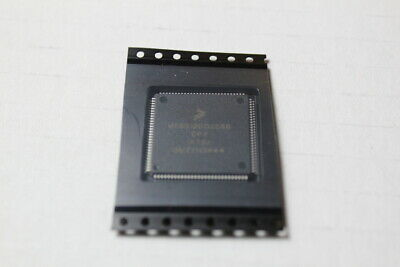
\includegraphics[scale=.4]{hcs12.jpg}

	\end{multicols}


}


% Section I
\section{\sectiontitleI}

	% Section I - Frame I
	\begin{frame}[label=sectionI,containsverbatim] \small
		\frametitle{\sectiontitleI}
	
		A microcontroller (MCU for microcontroller unit) is a small computer on a single metal-oxide-semiconductor (MOS) integrated circuit (IC) chip. A microcontroller contains one or more CPUs (processor cores) along with memory and programmable input/output peripherals.
	
		\begin{itemize}
			
			\item System on Chip
			
			\item Examples: 
			
			\begin{multicols}{2}
			\begin{itemize}
				
				\item Motorolla HCS12
				\item Pic
				\item Atmel Atmega 2560
				\item Atmel Atmega 328p
				\item STM32 Arm Cortex M0
				\item STM32 Arm Cortex M4
			\end{itemize}
			
			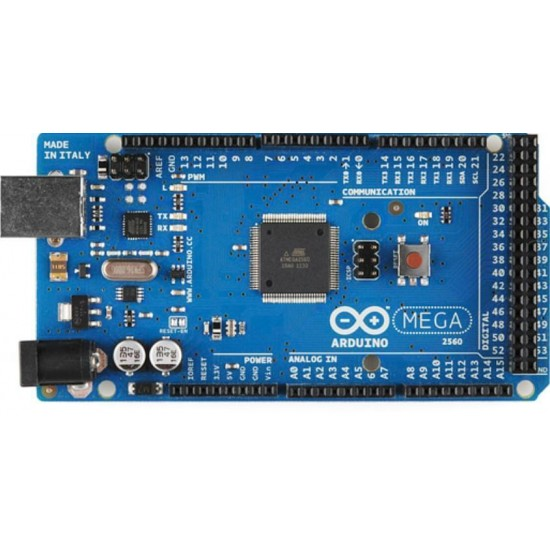
\includegraphics[scale=.2]{mega2560.jpg}
			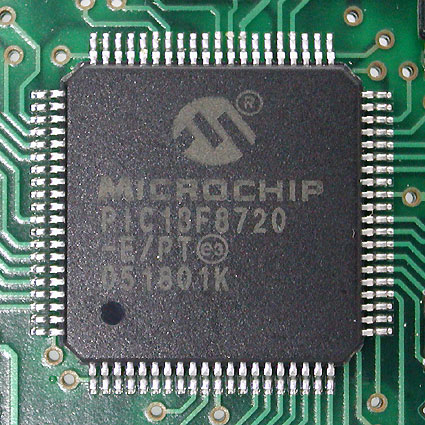
\includegraphics[scale=.1]{PIC18F8720.jpg}
			
			\end{multicols}
		\end{itemize}

	{\tiny \href{https://en.wikipedia.org/wiki/System_on_a_chip}{wikipedia - SoC} }

	\end{frame}


% Section II
\section{\sectiontitleII}

	% Section II - Frame I
	\begin{frame}[label=sectionII,containsverbatim] \small
		\frametitle{\sectiontitleII}

		Microcontrollers are used in embedded system design in many different systems...
		
		\begin{itemize}
			
			\item Automotive 
			\item Aerospace
			\item Personal Devices
			\item Appliances
			\item and many more ...
			
		\end{itemize}
		
		
	\end{frame}


% Section III
\section{\sectiontitleIII}

	\begin{frame}[label=sectionIII,containsverbatim] \small
	\frametitle{\sectiontitleIII}

	A microntoller is a system on a chip. \vspace{5mm}\\
	
	{\it A system on a chip (SoC...) is an integrated circuit (also known as a "chip") that integrates all or most components of a computer or other electronic system. These components almost always include a central processing unit (CPU), memory, input/output ports and secondary storage, often alongside other components such as radio modems and a graphics processing unit (GPU) – all on a single substrate or microchip. }

	\end{frame}

	\begin{frame}[label=sectionIII] \small
\frametitle{\sectiontitleIII}

		PIC12C508\\
		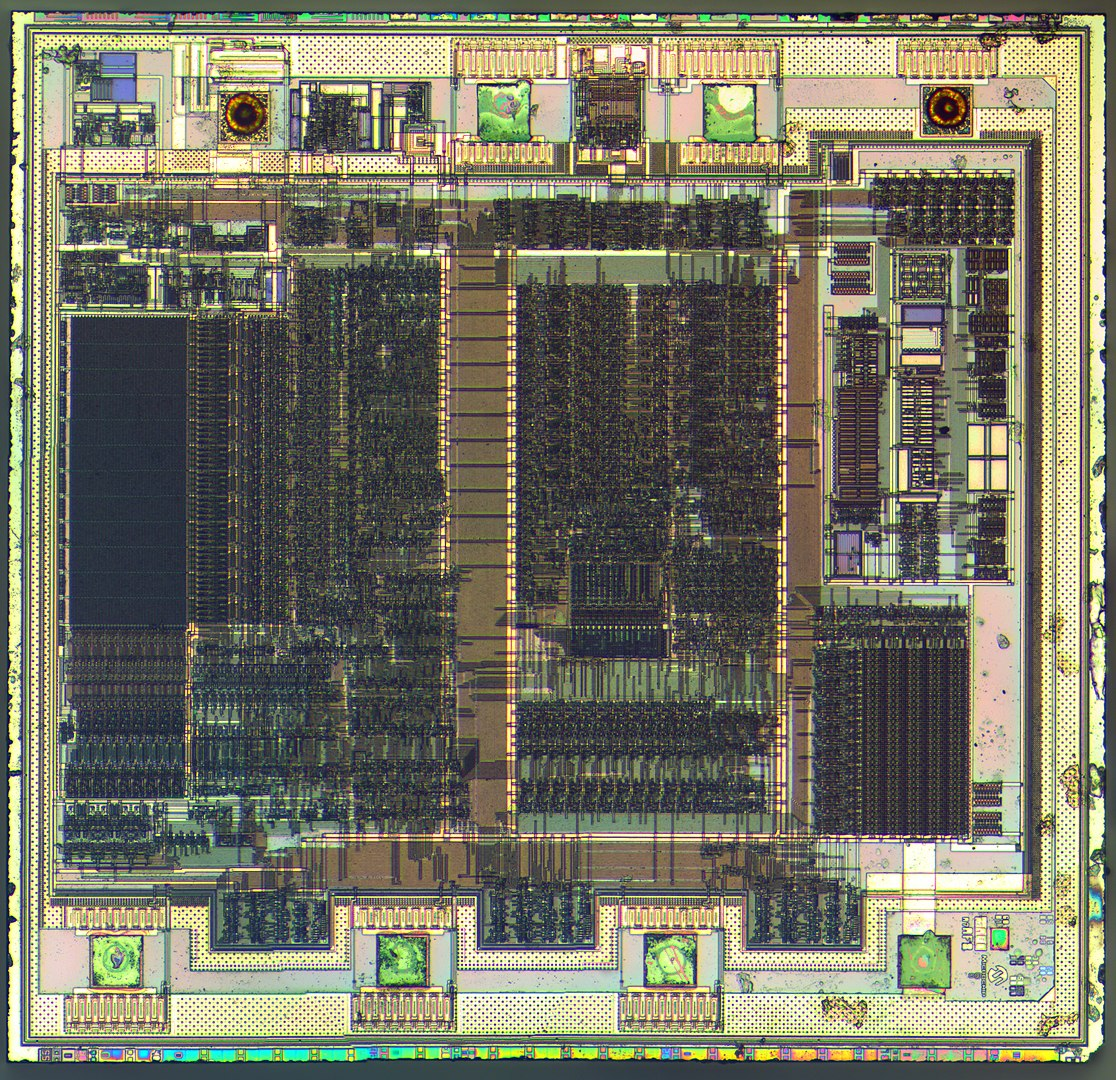
\includegraphics[scale=.15]{pic12c508_die_hd.png}



\end{frame}

	\begin{frame}[label=sectionIII] \small
\frametitle{\sectiontitleIII}


STM32 \\
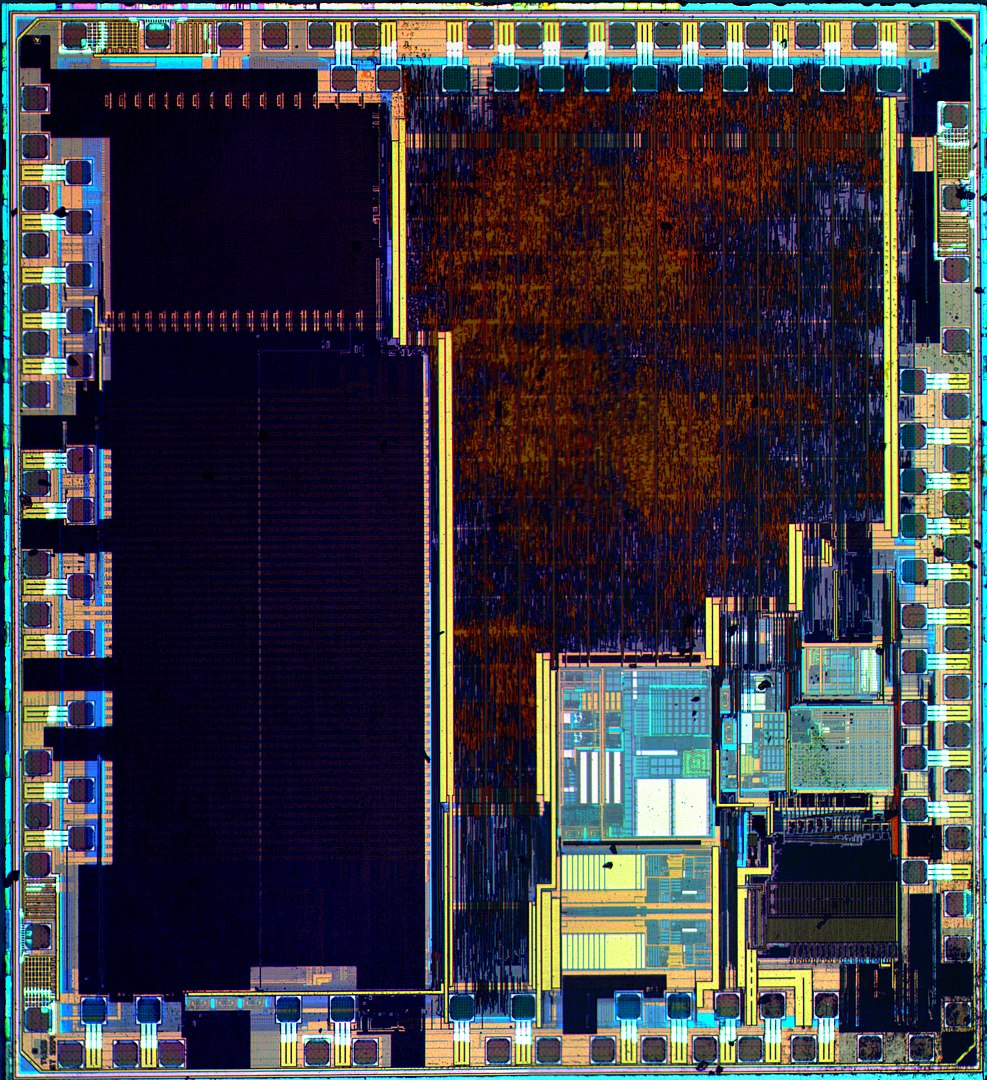
\includegraphics[scale=.15]{stm32_die.png}


\end{frame}



% Section IV
\section{\sectiontitleIV}	
	% Section IV - Frame I
	\begin{frame}[label=sectionIV,containsverbatim] \small
		\frametitle{\sectiontitleIV}    
	
		What does a MCU do that a desktop or notebook computer does not?
		
		\begin{itemize}
			
			\item
			\item
			\item
		\end{itemize}
	
	What does a desktop or notebook computer do that an MCU does not?
	
	\begin{itemize}
		
		\item
		\item
		\item
	\end{itemize}
		

		 

		\btVFill
		%\tiny{ref: \href{some link}{some text}} 
	\end{frame}

		% Section IV - Frame II
	\begin{frame}[label=sectionIV,containsverbatim] \small
	\frametitle{\sectiontitleIV}    
	
	\begin{itemize}
		\item CPU
		\item RAM
		\item ROM
		\item Oscillator
		\item GPIO 
		\item Peripherals 
		
	\end{itemize}

Example Datasheets: \href{https://components101.com/microcontrollers/atmega328p-pinout-features-datasheet}{atmel328p}
\href{https://www.nxp.com/docs/en/data-sheet/LPC8N04.pdf}{arm-cortex-m0}

	
	\btVFill
	\tiny{ref:} 
\end{frame}

% Section V
\section{\sectiontitleV}	
	% Section V - Frame I
	\begin{frame}[label=sectionV,containsverbatim] \small
	\frametitle{\sectiontitleV}    
	
	When programming a microcontroller, you use a {\BL cross compiler} built into the programming environment.
	

\end{frame}




\end{document}

